\section {Eksperymenty}
\subsection {Experyment pierwszy: pomieszczenie codziennego użytku}
Pierwszy z wykonanych eksperymentów polegał na wygenerowaniu obrazu pomieszczenia w którym pracowałem nad pisaną właśnie pracą dyplomową (salon z aneksem kuchennym).
Pomieszczenie ma XX metrów kwadratowych i znajdują się w nim elementy codziennego użytku - lodówka, zlew kuchenny, kwiaty na parapecie oraz otwór dzwiowy łączcy pomieszczenie z przedpokojem. Wymiary pokoju to XX m x XX m.\\


Dla opisanego pomieszczenia wygenerowany został następujący obraz:
\begin{figure}[h]
    \centering
    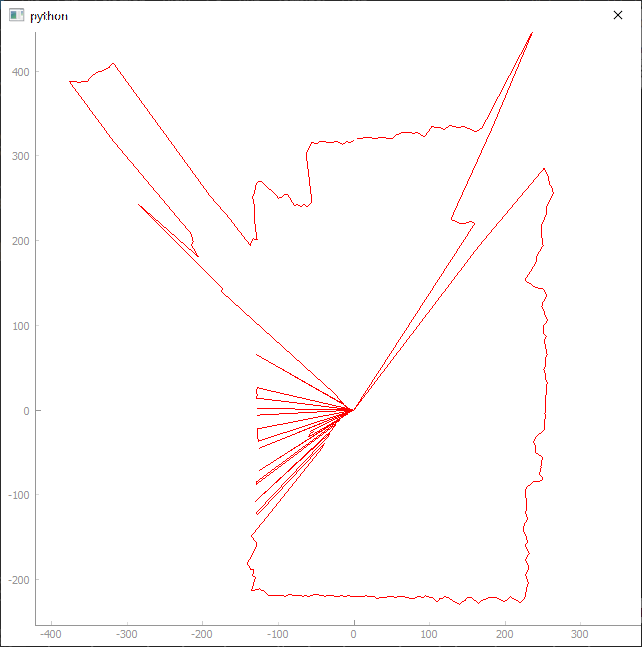
\includegraphics[scale=0.5]{experiment_1_plot}
    \caption{Wygenerowany obraz pomieszczenia - salonu z aneksem kuchennym}
    \label{fig:experiment_1_plot}
\end{figure}

W chwili generowania obrazu dalmierz znajdował się ok. 110 cm ponad powierzchnią podłogi, dzięki czemu nie znalazły się na nim stojące w pokoju umeblowanie.

\subsection {Experyment pierwszy: analiza wygenerowanego obrazu}

Wygenerowany obraz przedstawia dosyć wierne odwzorowanie badanego pomieszczenia. Ze względu na amatorski charakter urządzenia znalazło się w nim jednak kilka przekłamań:

\begin{enumerate}
    \item Otwór dzwiowy spowodował odczyt odległości do ściany w sąsiednim pomieszczeniu (przedpokoju) oraz kolejnym pokoju.
    \item Połyskująca powierzchnia lodówki wprodziła przekłamanie na jej frontowej powierzchni - wygenerowany jej obraz sprawia mylne wrażenie rombu. 
    \item Metalowy kran o obłym krztałcie prowadza kilka znieszkałceń - ze względu na refleksję promienia lasera.
    \item Na parapecie stoją doniczki z kwiatami co uwzględnione zostało na neregularnych kształtach wykresu
    \item Puste ściany z kąty proste odzwierciedlone zostały w dosyć dużą dokładnością.
    \item Ściana na przeciw okna została odzwierciedlola z kilkoma przekłananiami (odczyty zerowych wartości dalmierza). Powierzchnia w tym miejscu nie różni się niczym od pozostałch powierzni, zarówno użytą farbą, kolorem jak i nasłonecznieniem. Przyczyna błędnych wskazań w tym miejscu pozostaje nieznana.
\end{enumerate}

\newpage
\subsection {Experyment drugi: ocena użytej rodzielczości}

W drugim eksperymencie chciałem przekonać się o dokładności dalmierza i o tym czy zastosowana przez mnie rodzielczość (400 króków na pełen obrót) jest wystarczająca.\\

W tym celu wyłączyłem zasilanie silnika krokowego, przez co dalmierz zczytywał wciąż tę samą ogległość. Program jednak nadawał sygnał do zmiany kąta przez co przekonany był o obrocie silnika. W skutek tego otrzymaliśmy obraz okręgu (ta sama odległość dla "każdego" z kątów).

\begin{figure}[h]
    \centering
    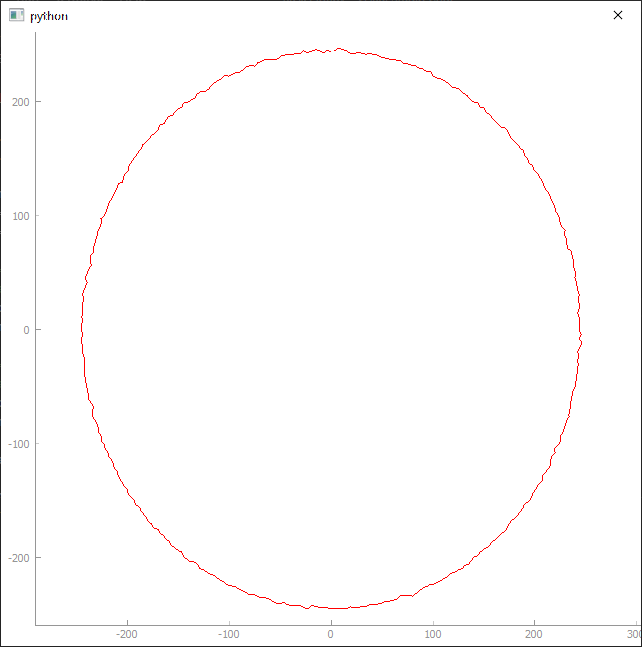
\includegraphics[scale=0.5]{experiment_2_plot}
    \caption{“Time is a flat circle” Friedrich Nietzsche}
    \label{fig:experiment_2_plot}
\end{figure}

\subsection {Experyment drugi: analiza wygenerowanego obrazu}

Wahania odczytów dalmierza różniły się od siebie z reguły o 1-2 cm, czasem o 3 cm. Wartość ta mieści się w podawanym w specyfikacji producenta zakresie.\\

Ilość wygenerowanych punktów (400) pozwoliła odzrować okrąd z bardzo dużą dokładnością. Krzywizna okręgu jest gładka a jej krztałt nie jest sprawia wrażenia widocznych pixeli (prostych linii wynikających ze zbyt rzadkiej siatki punktów). Nie ma potrzeby zwiększania rozdzielczości pracy urządzenia.\\
